\graphicspath{{01_introduction/figures/}} % Location of the graphics files

\chapter{Introduction}
\label{01_chp:introduction}

\section{The Common Grounding Problem}
\label{01_sec:common_grounding_problem}

Human communication is extraordinary. Unlike other primates, we use \textit{symbolic} natural language which can be assembled grammatically to express countless meanings, from abstract to concrete \citep{tomasello2009constructing}. Natural language is so versatile that most (if not all) of our knowledge is expressed, shared and elaborated through this medium. Hence, it is not surprising that such linguistic competence has been considered as a hallmark of human-level intelligence \citep{turing1950computing}.

But what makes human communication so reliable? At the heart of this question lies the problem of \textit{common grounding}. Common grounding is the process of creating and maintaining mutual understandings (i.e. \textit{common ground}), which is a critical aspect of sophisticated human communication. It is only through this collaborative effort that we can ensure the reliability of our shared understandings \citep{clark1996using}.

To illustrate how this process unfolds in natural language dialogues, we first introduce the \textit{contribution theory} of \citet{clark1989contributing}, which remains influential to date. According to this theory, information in dialogue transitions through 2 phases: the \textit{presentation phase}, where it gets first introduced by the speaker, followed by the \textit{acceptance phase}, where it gets acknowledged by the listener(s). It is only after the positive feedback from the listener(s) in the acceptance phase that the information is added (or \textit{contributed}) to their common ground.\footnote{Note that a piece of information can be presented in various ways, including direct assertions as well as indirect \textit{presuppositions}, e.g. implicitly assumed in a question \citep{stalnaker1978assertion}. Similarly, information can be accepted directly through acknowledgements (like ``yes'', ``okay'') or more indirectly, e.g. through the initiation of the next relevant contribution \citep{cho-may-2020-grounding}.}

To exemplify this process, we show an actual conversation reported in \citet{Sacks1974ASS}.

\ex. \label{ex_1:deictic_reference}
\a. A:\; Uh you been down \underline{here} before haven't you.
\b. B:\; Yeah.
\c. A:\; Where the sidewalk is?
\b. B:\; Yeah,
\e. A:\; Where it ends,
\f. B:\; Goes all the way up there?
\f. A:\; They come up to there, yeah.

In the first utterance (a), speaker A inquires whether B has been to the place (``\textit{here}'') before, which B recognizes and replies with a positive answer (b). These two utterances form a contribution, and the inquired fact becomes mutually accepted among A and B. However, there remains a potential ambiguity in the deictic reference ``here'', so the conversation continues to resolve it through clarifications and elaborations (c-g). Based on this process, the speakers can ensure the detail and reliability of common ground, and if there were any misunderstandings, they can be \textit{repaired} through correction (e.g. ``No, it's the \textit{opposite} side of the sidewalk.'') \citep{schegloff1977preference}.

Through the accumulation of this process, humans can develop a substantial amount of common ground foundational in various aspects of our daily life. Without the ability of reliable common grounding, the productive, stable and efficient collaboration in complex human society is unimaginable to be achieved.

%which plays a fundamental role in productive, efficient and reliable collaboration.% \citep{grosz1996collaborative,clark1996using}.

\section{Limitations of Existing Research}
\label{01_sec:existing_research}

The previous discussion corroborates the importance of common grounding in human communication. But how is this problem being addressed in the fields of artificial intelligence (AI) and natural language processing (NLP), and what are the main challenges that hinder its progress? Despite the long history of study on this topic, we raise three major limitations of existing research.

\subsubsection{Limitation on the Task Settings}

In dialogue research, \textit{task design} is an important factor that determines the subject of study (e.g. the complexity and requisite strategy of common grounding). However, existing dialogue tasks mostly focus on restricted domains and task settings where advanced, full-fledged common grounding is not required. To be specific, most existing tasks only need to deal with the following types of information which make the requisite skills of common grounding relatively trivial.

\begin{itemize}
\item \textit{Categorical} information: Traditionally, the type of information that dialogue systems handle has been limited to categorical/discrete information. For instance, the information of color would be discretized into predefined categories (e.g. ``red'', ``blue'', ``green'', and so forth) so that they can be treated with structured databases and frame-based dialogue state tracking \citep{Henderson2015}.

However, this setting ignores the aspect of many concepts being gradable and unbounded \citep{Lakoff87,paradis_2008} and introduces minimal ambiguity or uncertainty to be dealt with symbolic natural language. Consequently, they require minimal effort of semantic coordination (e.g. disambiguations and clarifications) in the process of common grounding.

\item \textit{Fully-observable} information: It is also common in prior works to assume that the information is fully-observable, i.e. all agents have the same, complete information of the environment. For instance, agents often have identical observations (e.g. the same set of images) to discuss in the dialogue \citep{zarriess-etal-2016-pentoref,de2017guesswhat,shore-etal-2018-kth}.

However, this assumption is unrealistic in many situations where we only have partial, private information of the environment. Due to the lack of such information asymmetry, existing settings introduce minimal misunderstandings or partial understandings that need to be resolved through common grounding.

\item \textit{Static} information: Finally, existing dialogue tasks mostly focus on static information and environments that do not change over time. For instance, dialogue contexts like databases \citep{he2017learning}, images \citep{haber-etal-2019-photobook} and embodied environments \citep{de2018talk,thomason:corl19} are usually assumed to be fixed/stationary in the course of the dialogue.

However, real-world environments are \textit{dynamic} and require continuous effort of maintaining common ground. In the static settings of existing works, there are minimal requirements for updating common ground and adapting to the evolving situations, e.g. by replacing old information with the new ones.

\end{itemize}

\subsubsection{Limitation on the Evaluation and Analysis}

Secondly, how to evaluate and analyze common grounding largely remains an open problem.
One main difficulty of evaluation is that systems can \textit{imitate} common grounding without actual understandings, either through simple acknowledgements and paraphrasing \citep{weizenbaum1966eliza} or based on more elaborate human-like responses \citep{adiwardana2020towards,roller-etal-2021-recipes}. Such deceptive behaviors could be misleading or even harmful to promote research on reliable common grounding. Another difficulty is the existence of \textit{dataset biases}. In the process of dataset creation, there could be various sources of suprious, unintended biases \citep{goyal2017making,gururangan-etal-2018-annotation,geva-etal-2019-modeling} which can be exploited by the models to succeed without employing the genuine, intended abilities \citep{geirhos2020shortcut}. To overcome these limitations, we need more objective, quantitative and faithful evaluation metrics to measure and propel our real progress on advanced common grounding.

In terms of analysis, there are various factors that make the analysis of common grounding difficult or problematic in realistic settings. For instance, the application of \citeauthor{clark1989contributing}'s theory may not be straightforward when contributions are implicit, indirect, unstructured, partial, etc. To illustrate this, we use another example from \citet{Sacks1974ASS}, following the explanations of \citet{lascarides2009agreement}.

\ex. \label{ex_2:event_reference}
\a. Mark (to Karen and Sharon):\; Karen `n I're having a fight,
\b. Mark (to Karen and Sharon):\; after she went out with Keith and not me.
\c. Karen (to Mark and Sharon):\; Well Mark, you never asked me out.

In this dialogue, Mark and Karen agree on the fact that the \textit{cause} of the fight was Karen going out with Keith: however, this is only presented through an \textit{implicature} in Mark's utterances (from the ``fight'' occurring after Karen ``went out with Keith''). Furthermore, Karen accepts this without direct acknowledgement, but instead through the initiation of a relevant contribution (i.e. the \textit{explanation} of why she went out with Keith). This suggests that both the presentation and acceptance phase of the contribution can be implicit and difficult to identify in actual conversations. Hence, we need more reliable methods to interpret and analyze the intermediate process of common grounding.

\subsubsection{Limitation on the Model Capability}

Finally, we raise the limitation of the model capability for sophisticated common grounding. Generally speaking, there are two mainstream approaches in building contemporary dialogue systems \citep{gao2019neural}. The first approach is the so-called \textit{traditional} approach, where the dialogue system is carefully designed as a pipeline of specialized modules. In this approach, each module would be responsible for a certain subprocess of dialogue, such as parsing user utterances \citep{yao2013recurrent}, tracking dialogue states \citep{henderson-etal-2014-word}, planning next utterances \citep{peng-etal-2017-composite} and realizing their surface forms \citep{wen-etal-2015-semantically}. While this approach has the advantage of being more interpretable, controllable and robust to expectable errors, the reliance on manual design (e.g. on the modularization) becomes a bottleneck in achieving scalability, generality and flexibility required for human-level common grounding.

The second approach is the so-called \textit{end-to-end} approach, where the dialogue system is developed in a fully data-driven manner with minimal prior constraints, typically using the neural networks \citep{vinyals2015neural,bordes2017learning}. As long as sufficient/appropriate data are available, this approach has the advantage of being more scalable, flexible and applicable to general domains: in fact, even to the most challenging \textit{open domains} as required for the chatbots \citep{adiwardana2020towards,roller-etal-2021-recipes}. However, the major drawback is the lack of interpretability, controllability and robustness to recover in the face of even trivial mishaps arising from miscommunication \citep{brennan1998grounding,benotti-blackburn-2021-grounding}.

Therefore, incorporating human design (first approach) and learning directly from data (second approach) have complementary strengths/weaknesses, and neither is sufficient by itself. While there are recent approaches that aim the ideal middle ground \citep{williams-etal-2017-hybrid,andreas-etal-2020-task}, realizing human-level common grounding (e.g. in terms of both flexibility and robustness) still remains an open challenge.

\section{Contributions of the Thesis}
\label{01_sec:contributions}

\begin{figure*}[t!]
\centering
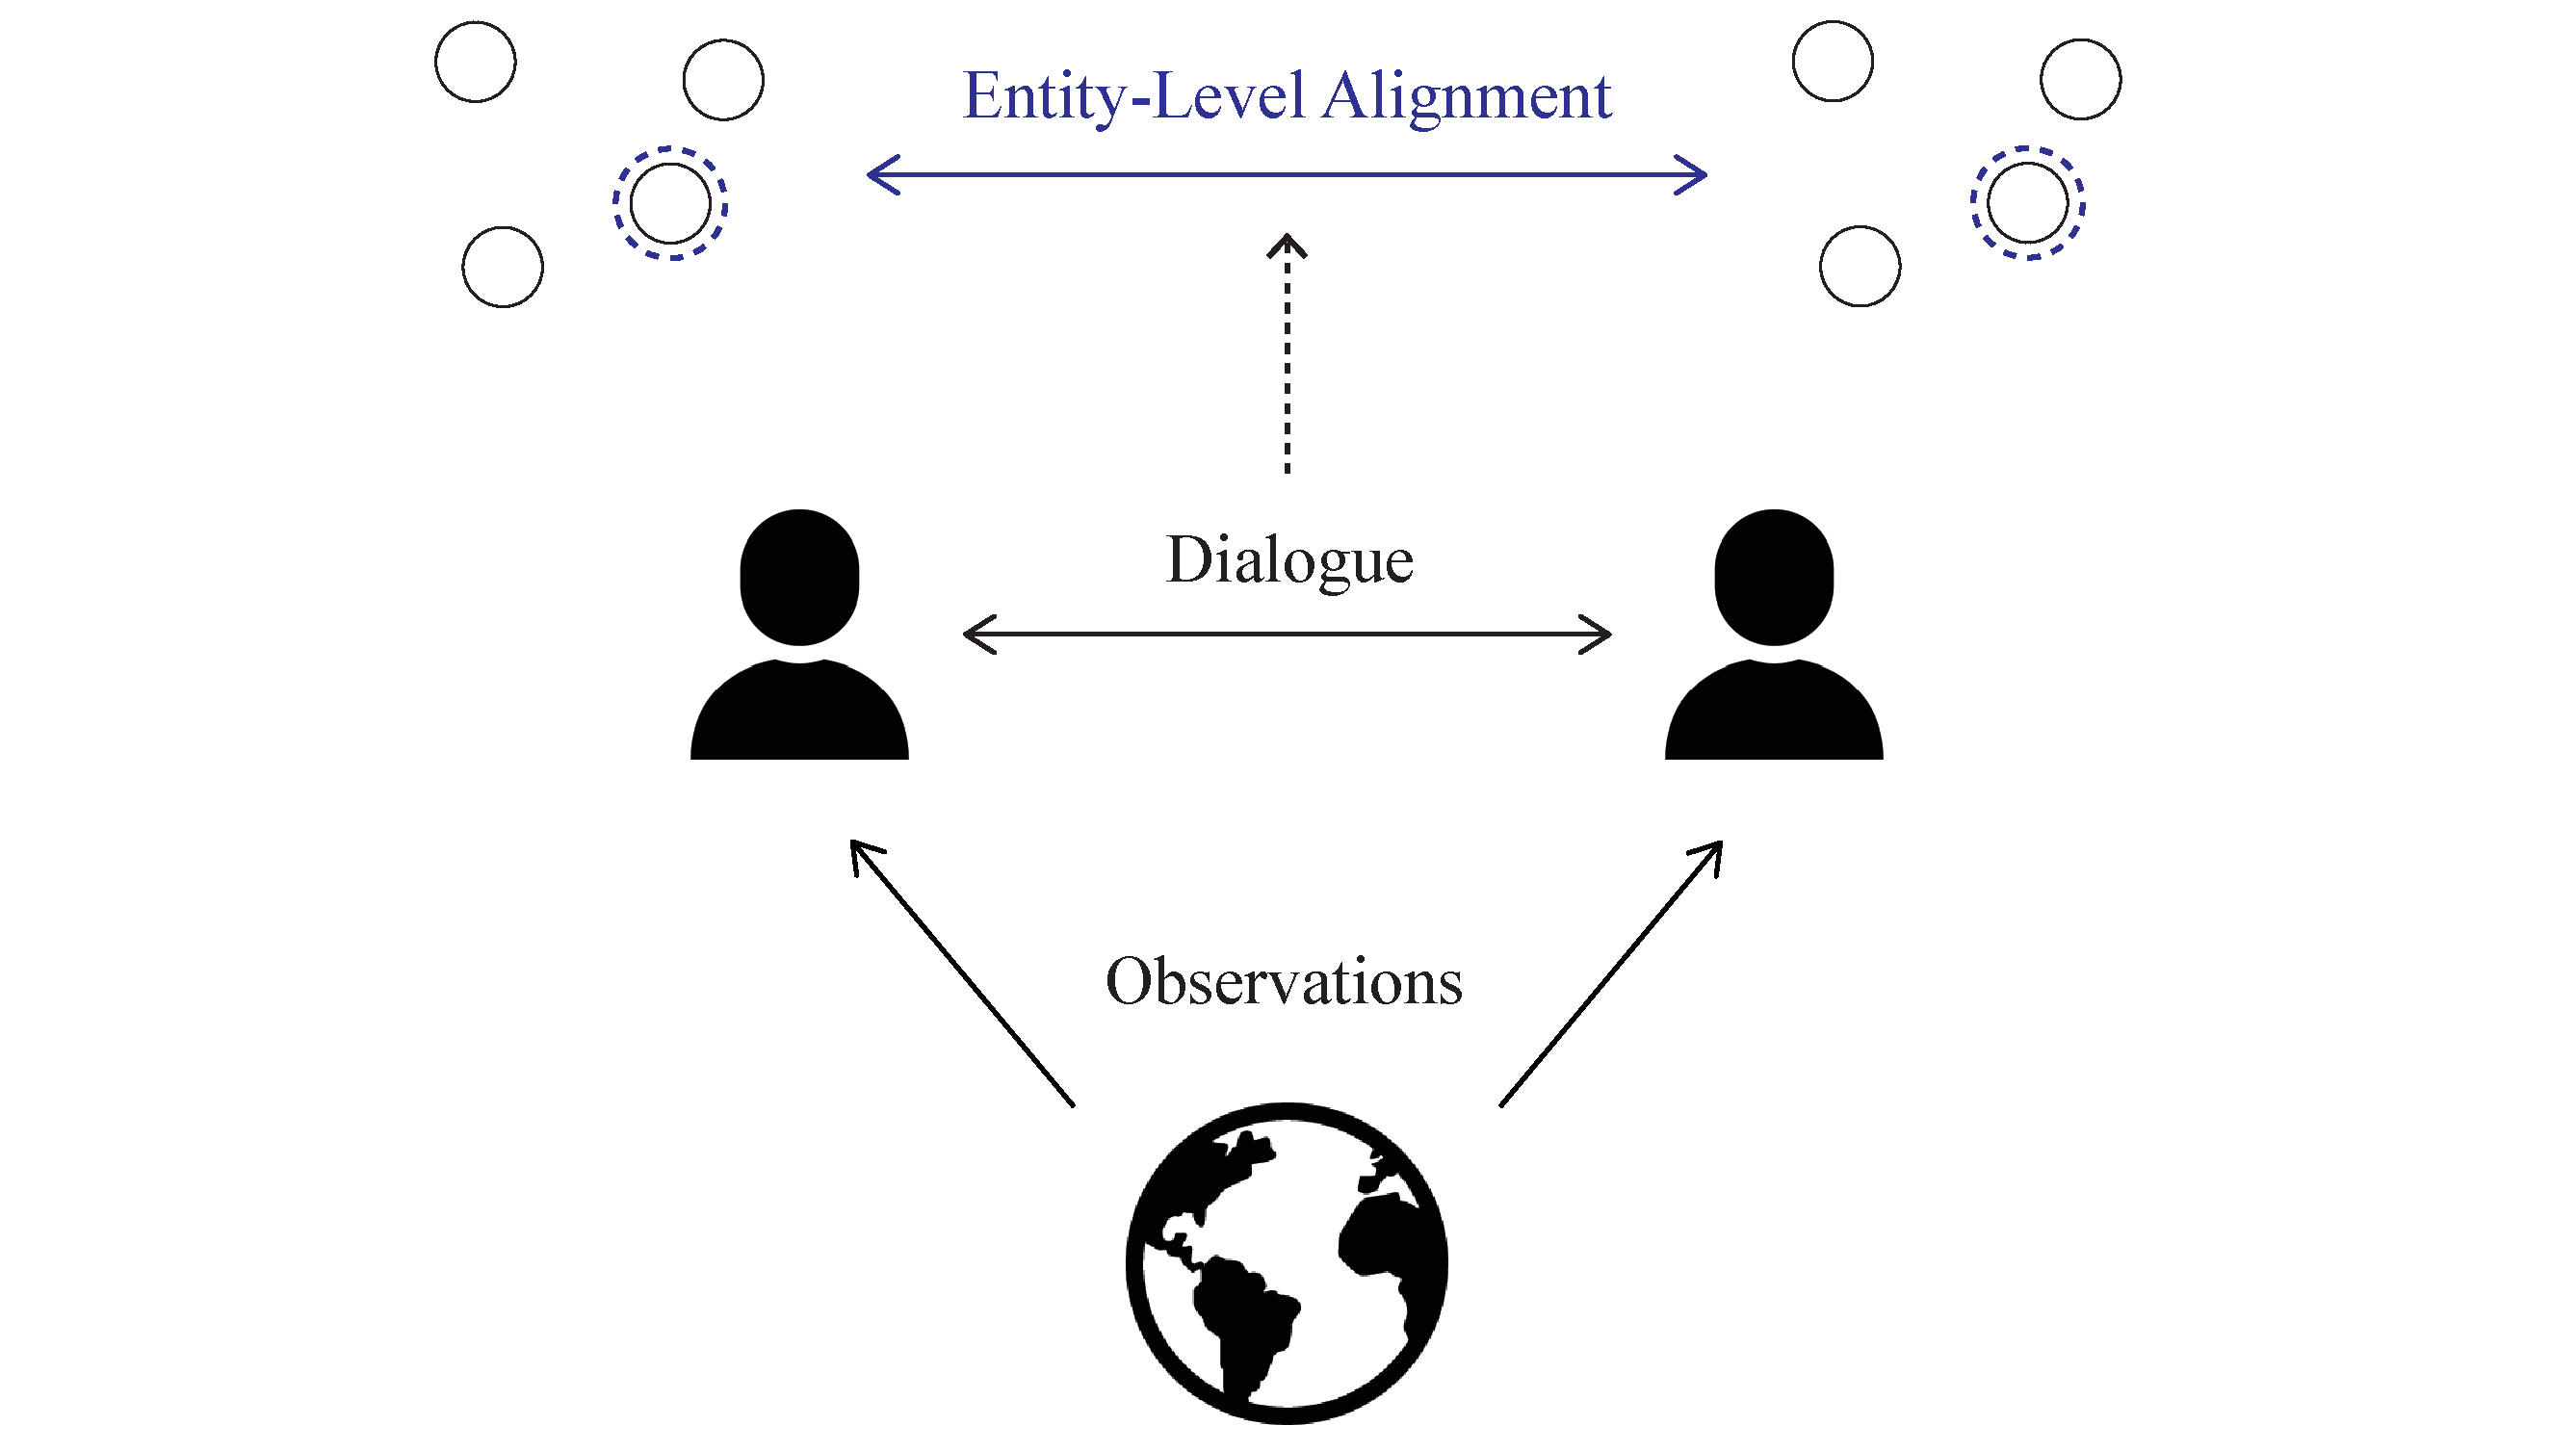
\includegraphics[width=\textwidth]{entity_level_alignment.pdf}
\caption{An illustration of our task formulation as \textit{entity-level alignment}.
}
\label{01_fig:entity_level_alignment}
\end{figure*}

To address all of these problems, we propose a novel research platform to study advanced common grounding in natural language dialogue systems. To make the scope of this thesis precise, we focus on the aspect of \textit{entity-level alignment} as the critical first step in general common grounding. As visually depicted in Figure \ref{01_fig:entity_level_alignment}, this step can be formalized as the following dialogue process:

\begin{enumerate}
  \item First, we assume that each speaker has a private \textit{observation} of the environment. This can be respresented as a personal experience, knowledge, perception, etc, typically involving multiple entities in the environment.

  \item Secondly, the speakers converse in natural language to recognize the same entity in the environent. The type of entity to be recognized can vary depending on the objective, e.g. physical objects, locations, or temporal events. 

  \item Finally, we consider common grounding to be \textit{successful} if and only if the speakers could recognize the same entity. In other words, we consider common grounding to be an accurate \textit{alignment} of the private observations at the \textit{entity-level}.
\end{enumerate}

For instance, the example dialogue \ref{ex_1:deictic_reference} can be considered as the alignment of a \textit{locational} entity and example \ref{ex_2:event_reference} as the alignment of an \textit{event} (or possibly its \textit{cause}). While this formalization is simplified and ignores the aspect of entire common grounding, entity-level alignment is a critical and indispensable step in any type of common grounding, e.g. developing common ground of an entire scenery \citep{das2017visual,haber-etal-2019-photobook,alamri2019audio}.

By restricting our scope to this preliminary setting, we address each of the three major limitations in the following ways.

\subsubsection{Contribution on the Task Settings}

\begin{figure*}[t!]
\centering
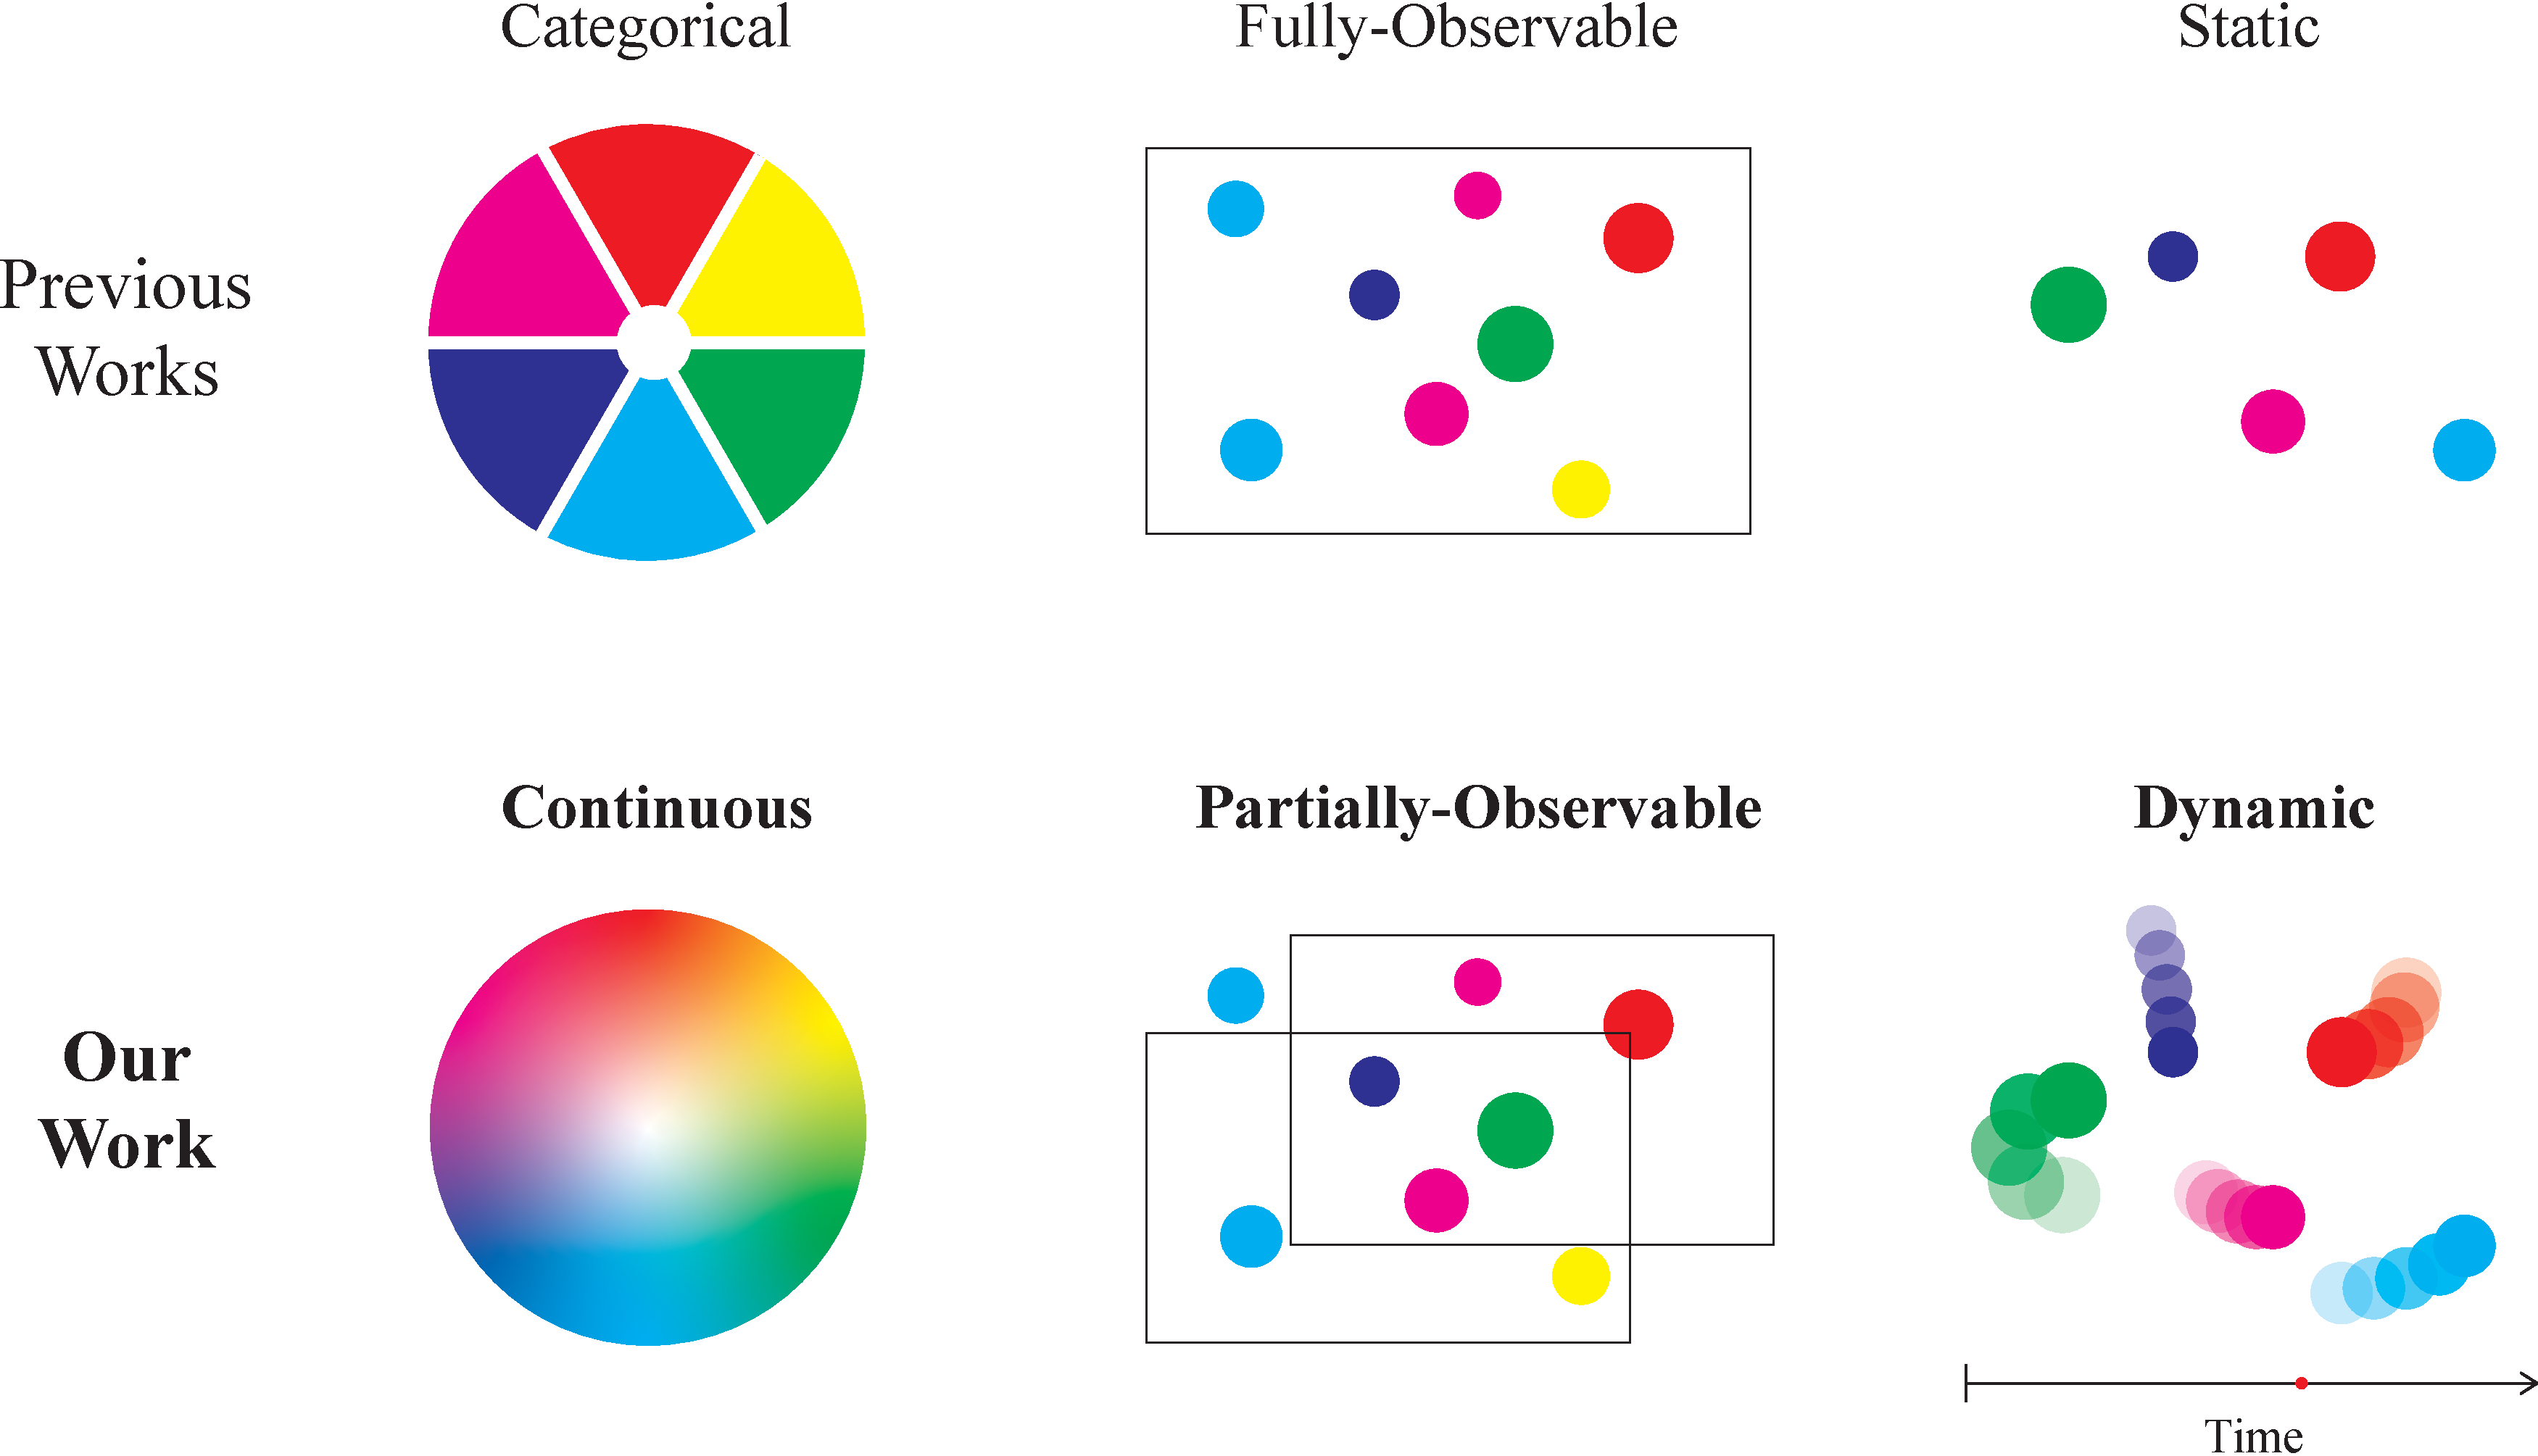
\includegraphics[width=\textwidth]{task_design.pdf}
\caption{An illustration of the task settings in previous works (top row) and our work (bottom row). We introduce \textit{continuity} to require more semantic coordination, \textit{partial observability} to require the resolution of potential misunderstandings, and \textit{dynamics} to incorporate the aspect of maintaining/updating common ground.
}
\label{01_fig:task_design}
\end{figure*}

We propose a novel task setting under \textit{continuous}, \textit{partially-observable} and (optionally) \textit{dynamic} context to require advanced skills of common grounding: see Figure \ref{01_fig:task_design} for a visual illustration in comparison to the previous settings. To be specific, we represent the dialogue context based on \textit{continuous} real values, which reflects the information (e.g. perception) in the physical world more faithfully and requires more advanced coordination, e.g. based on nuanced expressions \citep{paradis_2008} and pragmatic reasoning \citep{monroe2017colors}. In addition, we introduce \textit{partial-observability} where the agents have different perspectives of the environment, which is more realistic and requires to take into account the possibility of various misunderstandings \citep{keysar2000taking}. Finally (as an optional setting), we incorporate diverse \textit{dynamics} of the environments to require advanced skills of maintaining common ground: concretely, we incorporate dynamic scenes based on animations to require spatio-temporal reasoning \citep{girdhar2020cater} as well as information updates to require adaptation to the changing environments \citep{moon-etal-2020-situated}.

It is worth noting that each of these settings has been explored at least partially or independently in the previous literature: for instance, \citet{de2017guesswhat} proposed a reference game under \textit{continuous} visual context, and \citet{he2017learning} worked on a \textit{partially-observable} setting. However, our important contributions are the \textit{abstraction} of the task settings in the three universal dimensions and their \textit{combinations} to require more advanced common grounding. Owing to this level of abstraction, we can empirically investigate the consequences of each task setting in a scientific manner (i.e. through controlled experiments and hypothesis testing) and expect our findings to be general and fundamental for designing experimental setups in future dialogue research.


\subsubsection{Contribution on the Evaluation and Analysis}

\begin{figure*}[t!]
\centering
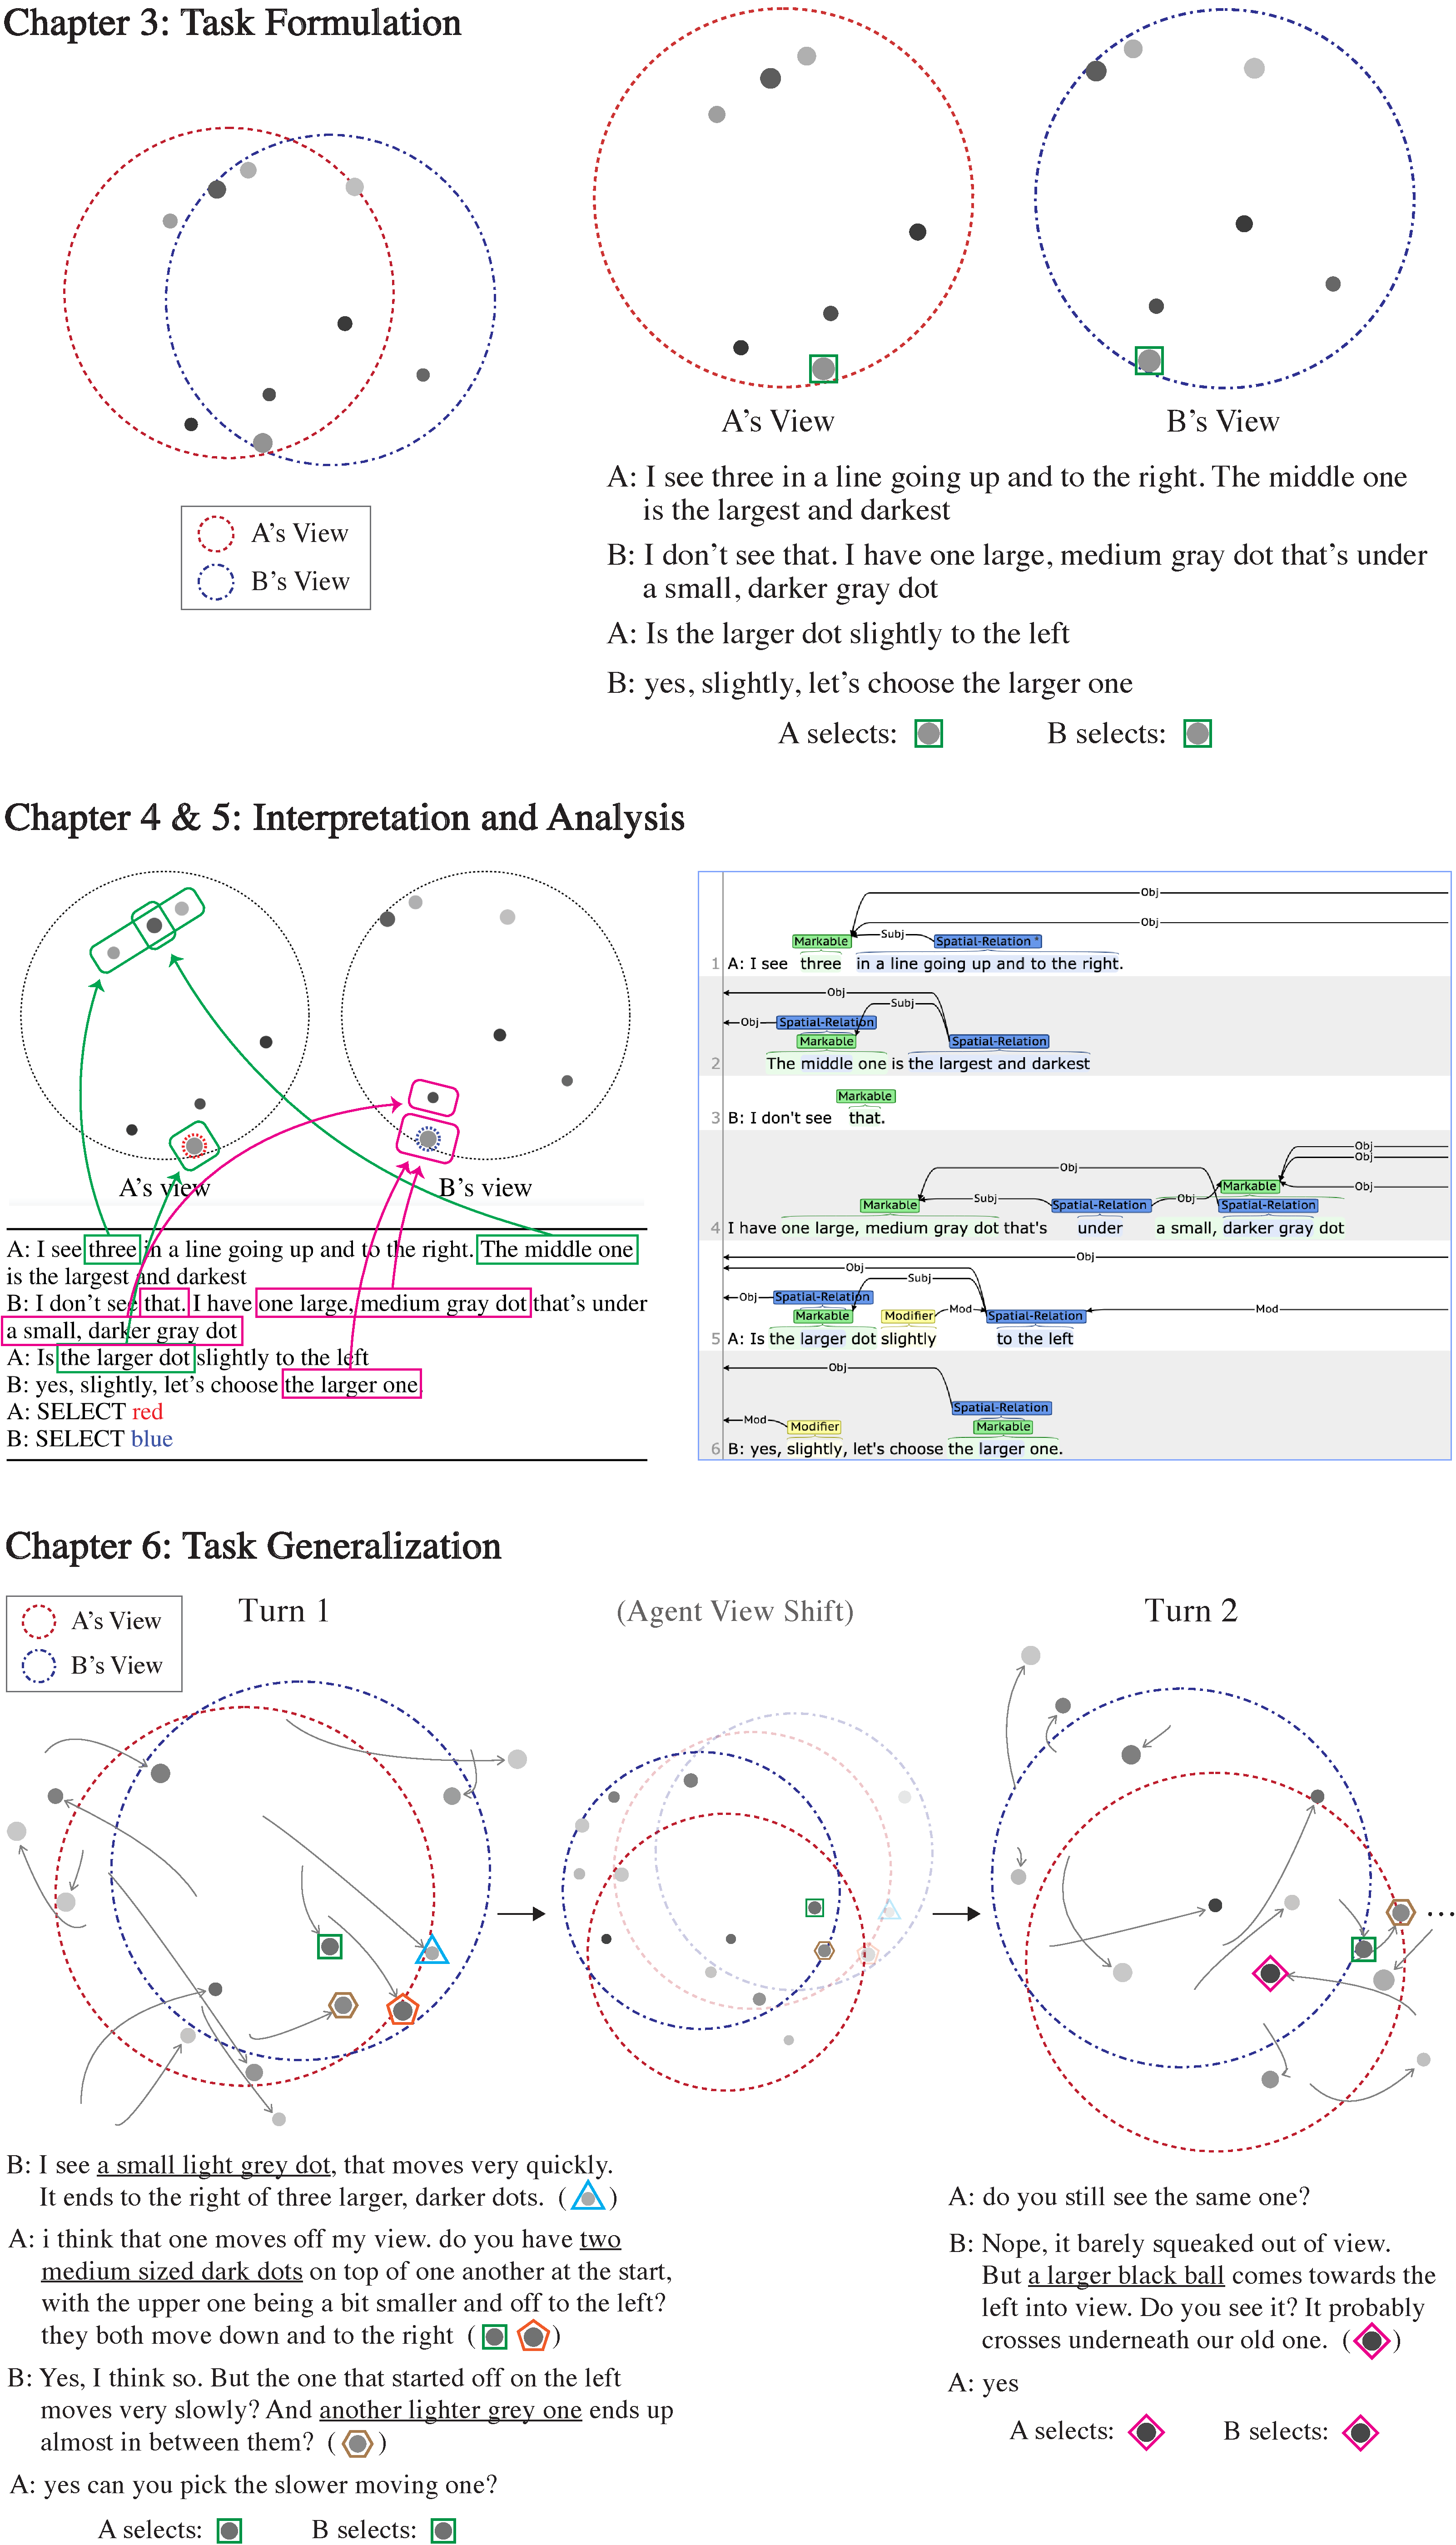
\includegraphics[width=\textwidth]{contribution_overview.pdf}
\caption{An overview of our task formulations and analytical frameworks.}
\label{01_fig:contribution_overview}
\end{figure*}

To evaluate the ability of creating common ground, we formulate a novel \textit{collaborative reference task}, where the goal of the agents is to select (i.e. coordinate attention on) the same entity through natural language dialogue. We consider this as an important step in general common grounding, since the mutual recognition of discourse entities (i.e. \textit{entity-level alignment}) is a fundamental building block in successful communication. Under this task formulation, we can evaluate the ability of accurate common grounding based on the \textit{task success rate}, which is both quantitative and objective. We also focus on a \textit{synthetic} environment to control, balance and diversify the dialogue contexts: this way, we can minimize undesirable biases and enable more faithful evaluation \citep{johnson2017clevr,girdhar2020cater}. We show an example dialogue of our collaborative reference task under \textit{continuous} and \textit{partially-observable} (but not \textit{dynamic}) context in Figure \ref{01_fig:contribution_overview} (top), which will be formally introduced in Chapter \ref{03_chp:task_formulation}.\footnote{Note that we also kept the \textit{task complexity} minimal for the ease of analysis.}

To analyze the process of common grounding, we propose a simple, reliable and useful framework of linguistic annotations. Specifically, we first identify the \textit{referring expressions} in the dialogue and the corresponding \textit{referent entities}, which can be in another modality (such as vision). This allows us to interpret the intermediate process of common grounding, such as how misunderstandings are introduced and resolved. Secondly, we conduct additional annotations to capture the detailed strategies of common grounding, such as how referring expressions are predicated or omitted in ellipses. To this end, we focus on \textit{spatial expressions} which are prevalent in visually grounded dialogues (including our own). We show an illustration of our analytical framework in Figure \ref{01_fig:contribution_overview} (middle), which will be discussed in detail in Chapter \ref{04_chp:interpretation} and \ref{05_chp:analysis}. Note that our analyses span different modalities (language and vision), which allow for investigating the related and important problem of \textit{symbol grounding} (c.f. Section \ref{02_sec:symbol_grounding}).

Under dynamic context, the collaborative reference task can be temporarily generalized to track and select the same entity at \textit{multiple timesteps} in the same environment: we refer to this as the \textit{sequential} collaborative reference task. Under this task formulation, we can further evaluate the ability of \textit{maintaining} accurate common ground based on the length of successful timesteps. We show an example dialogue of our sequential collaborative reference task in Figure \ref{01_fig:contribution_overview} (bottom), which will be formally introduced in Chapter \ref{06_chp:task_generalization}.

Based on the proposed task formulations and analytical frameworks, we enable reliable evaluation and detailed analysis of the fundamental aspects of common grounding.

\subsubsection{Contribution on the Model Capability}

Following the above ideas, we developed a collection of large-scale resources to train, evaluate and analyze various dialogue systems in terms of advanced common grounding. To be specific:

\begin{itemize}
  \item First, we collected 6,760 dialogues based on our minimal collaborative reference task under \textit{continuous} and \textit{partially-observable} context (Figure \ref{01_fig:contribution_overview}, top): we refer to this as OneCommon Corpus. Based on this dataset, we evaluate our baseline model's capability of \textit{recognizing} the created common ground in Chapter \ref{03_chp:task_formulation}.

  \item Secondly, we curated 5,191 successful dialogues from OneCommon Corpus and conducted the annotation of reference resolution (Figure \ref{01_fig:contribution_overview}, middle left). We describe how this resource can be leveraged to interpret and improve the common grounding strategies of our baseline model in Chapter \ref{04_chp:interpretation}.

  \item Thirdly, we randomly sampled 600 dialogues (already annotated with reference resolution) and further conducted the annotation of spatial expressions (Figure \ref{01_fig:contribution_overview}, middle right). Based on this annotation, we assess how well our improved baseline can recognize the fine-grained linguistic structures of the visually-grounded dialogues in Chapter \ref{05_chp:analysis}.

  \item Finally, we collected additional 5,617 dialogues based on our sequential collaborative reference task under \textit{continuous}, \textit{partially-observable} and \textit{dynamic} context (Figure \ref{01_fig:contribution_overview}, bottom): we refer to this as Dynamic-OneCommon Corpus. Based on this dataset, we assess our baseline model's capability of creating, retaining and updating common ground in dynamic environments in Chapter \ref{06_chp:task_generalization}.
\end{itemize}

In this thesis, we mainly focus on the simple and widely used \textit{end-to-end} dialogue systems \citep{vinyals2015neural,bordes2017learning,lewis-etal-2017-deal} as our baselines. However, our platform can be leveraged to experiment with various other approaches, as we discuss in Section \ref{02_sec:dialogue_systems}. While we leave further model assessments and improvements as future work, we propose a fundamental testbed for evaluating, analyzing and improving dialogue systems in terms of advanced common grounding.
\\

To summarize our contributions, we proposed novel task settings to study advanced common grounding as entity-level alignment. Based on our careful task designs, we formulated the (sequential) collaborative reference tasks to evaluate the ability of creating and maintaining accurate common ground. We also proposed useful analytical frameworks to interpret and analyze the intermediate process of common grounding. Finally, we developed large-scale resources for conducting various empirical studies, including the evaluation, analyses and improvements of data-driven dialogue systems.

Overall, we expect our proposed platform to be fundamental for promoting research on advanced common grounding in natural language dialogue systems.


\section{Thesis Outline}
\label{01_sec:thesis_outline}

The outline of this thesis is as follows:

\begin{itemize}
  \item In Chapter \ref{02_chp:literature_review}, we give an overview of the existing literature related to common grounding. This includes its theoretical foundations, computational research, and relationship with symbol grounding approached within various fields. Whenever appropriate, we clarify/explicate the novelty, motivations and contributions of this thesis to place them in these broader contexts.

  \item In Chapter \ref{03_chp:task_formulation}, we introduce a novel collaborative reference task under \textit{continuous} and \textit{partially-observable context}. Based on this task formulation, we collected 6,760 dialogues through crowdsourcing, which we refer to as OneCommon Corpus. Through our dataset analysis and experiment, we verified the advanced common grounding strategies required in this setting as well as the open room left for improvement. This chapter is based on our published work \citep{udagawa2019natural}.

  \item In Chapter \ref{04_chp:interpretation}, we propose a method of interpreting common grounding based on \textit{reference resolution}. Based on our novel framework, we annotated 5,191 dialogues from OneCommon Corpus via a combination of expert annotators and crowd workers. Our dataset analysis and experiment demonstrate the advantages of our annotation for interpreting the intermediate process of common grounding. This chapter is based on our published work \citep{udagawa2020annotated}.

  \item In Chapter \ref{05_chp:analysis}, we conduct further analyses by leveraging the existing annotation (reference resolution) to annotate \textit{spatial expressions}. We capture fine-grained linguistic structures of 600 dialogues in OneCommon Corpus, including predicate-argument structure, modification and ellipsis. Based on our improved baseline, we run a comprehensive assessment of the model's capability for recognizing such structures. This chapter is based on our published work \citep{udagawa-etal-2020-linguistic}.

  \item In Chapter \ref{06_chp:task_generalization}, we propose a novel task setting under \textit{dynamic} context to study the ability of mainining common ground. Based on our \textit{sequential} collaborative reference task, we crowdsourced 5,617 human dialogues, which we refer to as Dynamic-OneCommon Corpus. Through our dataset analysis and experiment, we demonstrate even more sophisticated strategies required in this setting in comparison to the \textit{static} counterpart of OneCommon Corpus. This chapter is based on our work to be published \citep{udagawa2021maintaining}.

  \item In Chapter \ref{07_chp:discussion}, we discuss the promising directions worth exploring in future research. Specifically, we propose further ideas on the \textit{task design methodologies} to require fully advanced common grounding, \textit{model improvements} to achieve more flexible and robust common grounding, and \textit{real-world applications} that naturally follow from the studies in this thesis.
\end{itemize}

